%\pdfobjcompresslevel=0
%\pdfminorversion=4
\documentclass[aspectratio=43]{beamer}

\usepackage{hyperref}
\usepackage{multimedia}
\usepackage{subfigure}
\usepackage[textsize=tiny]{todonotes}
\usepackage{tabu}
\usepackage{graphicx}
\presetkeys%
{todonotes}%
{inline}{}


%\usepackage[pdftex]{graphicx}
%\usepackage{graphviz}
\usepackage{graphviz}
%===Pick Theme===
\usetheme{Warsaw}
\usecolortheme{beaver}
\useoutertheme{infolines}
\useinnertheme{circles}

%===Customize Theme=== %
\setbeamercolor{item}{fg=darkred}
\setbeamertemplate{itemize subitem}{$\circ$}
\setbeamercolor*{block title}{fg=white, bg=darkred}
\setbeamercolor*{block body}{bg=lightgray}

%===Set the covered style=== %
\setbeamercovered{transparent}
%===Set the bib reference key style=== %
\setbeamertemplate{bibliography item}[text]
%===Disable navigation bar=== %
\setbeamertemplate{navigation symbols}{}%remove navigation symbols

\usepackage{minted}
\setminted[python]{bgcolor=bg,fontsize=\scriptsize,linenos,xleftmargin=8pt}
\setminted[xml]{bgcolor=bg,fontsize=\scriptsize,linenos,xleftmargin=8pt}

\setmintedinline[python]{bgcolor=bg,fontsize=\scriptsize}
\setmintedinline[bash]{bgcolor=bg,fontsize=\scriptsize}
\setmintedinline[text]{bgcolor=bg,fontsize=\scriptsize}
\setmintedinline[xml]{bgcolor=bg,fontsize=\scriptsize}

\newcommand{\pyinline}[1]{\mintinline{python}{#1}}
\newcommand{\bashinline}[1]{\mintinline{bash}{#1}}
\newcommand{\inline}[1]{\mintinline{text}{#1}}
%===Logos=== %

%\usepackage{pgf}
%\logo{\pgfputat{\pgfxy(-1,7)}{\pgfbox[center,base]{
\includegraphics[height=0.5in]{fig/duckietown_logo}}}}

\logo{
\includegraphics[height=0.5in]{fig/duckietown_logo}}
\titlegraphic{ %
\centering

\includegraphics[height=1.6in]{fig/duckietown_logo}%\hspace{2ex}
%\raisebox{-0.75in}{
\includegraphics[height=1.5in]{fig/indigoigloo_600.png}}
} %

% \author[Michael ``Misha'' Novitzky]{Michael ``Misha'' Novitzky}
\author[S.-Y.Liu, M. Novitzky]{Shih-Yuan Liu and Michael ``Misha'' Novitzky}
\title[ROS in Duckietown]{Middleware, Software Architecture, and ROS in Duckietown}
\institute[Duckietown MIT]{Duckietown, MIT}
\date[Feb. 17th, 2016]{February 17th 2016}



\begin{document}
\definecolor{bg}{rgb}{0.95,0.95,0.95}


\begin{frame}[plain,label=titlepage,noframenumbering] %[plain,noframenumbering] will not show the header and footer
	\titlepage
\end{frame}


%\begin{frame}{Intended Learning Outcome}
%	\begin{block}{Learning Objectives}
%		\begin{itemize}[<+->]
%			\item Describe the value of middleware for robotics software development
%			\item Answer the question: ``What is your favorite robotics middleware and why is it ROS?''
%			\item Draw computation graph for simple robotic system using publish/subscribe model
%			\item Explain important ROS concepts such as node, topic, message, and parameters
%			\item Use important ROS command-line tools
%			\item Write a simple ROS node by following code examples
%		\end{itemize}
%	\end{block}
%\end{frame}

\section{Introduction to Middlewares}

%\begin{frame}{Duckiebot Videos}
%\begin{columns}
%	\begin{column}{0.55\textwidth}
%		Shih-Yuan - how do I embed \alert{videos} in latex? Probably not right? Output is PDF. \todo{See videos slide}
%		\begin{itemize}
%			\item Output line filter?
%			\item Open-loop intersection?
%			\item Lane following awesomeness -- for sure
%		\end{itemize}
%	\end{column}
%	\begin{column}{0.45\textwidth}
%		\centering
%		
\includegraphics[width=\textwidth]{fig/indigoigloo_600.png}
%	\end{column}
%\end{columns}
%\end{frame}

\begin{frame}{Duckiebot Lane Following in Action}
\begin{center}
	\movie[showcontrols=true]{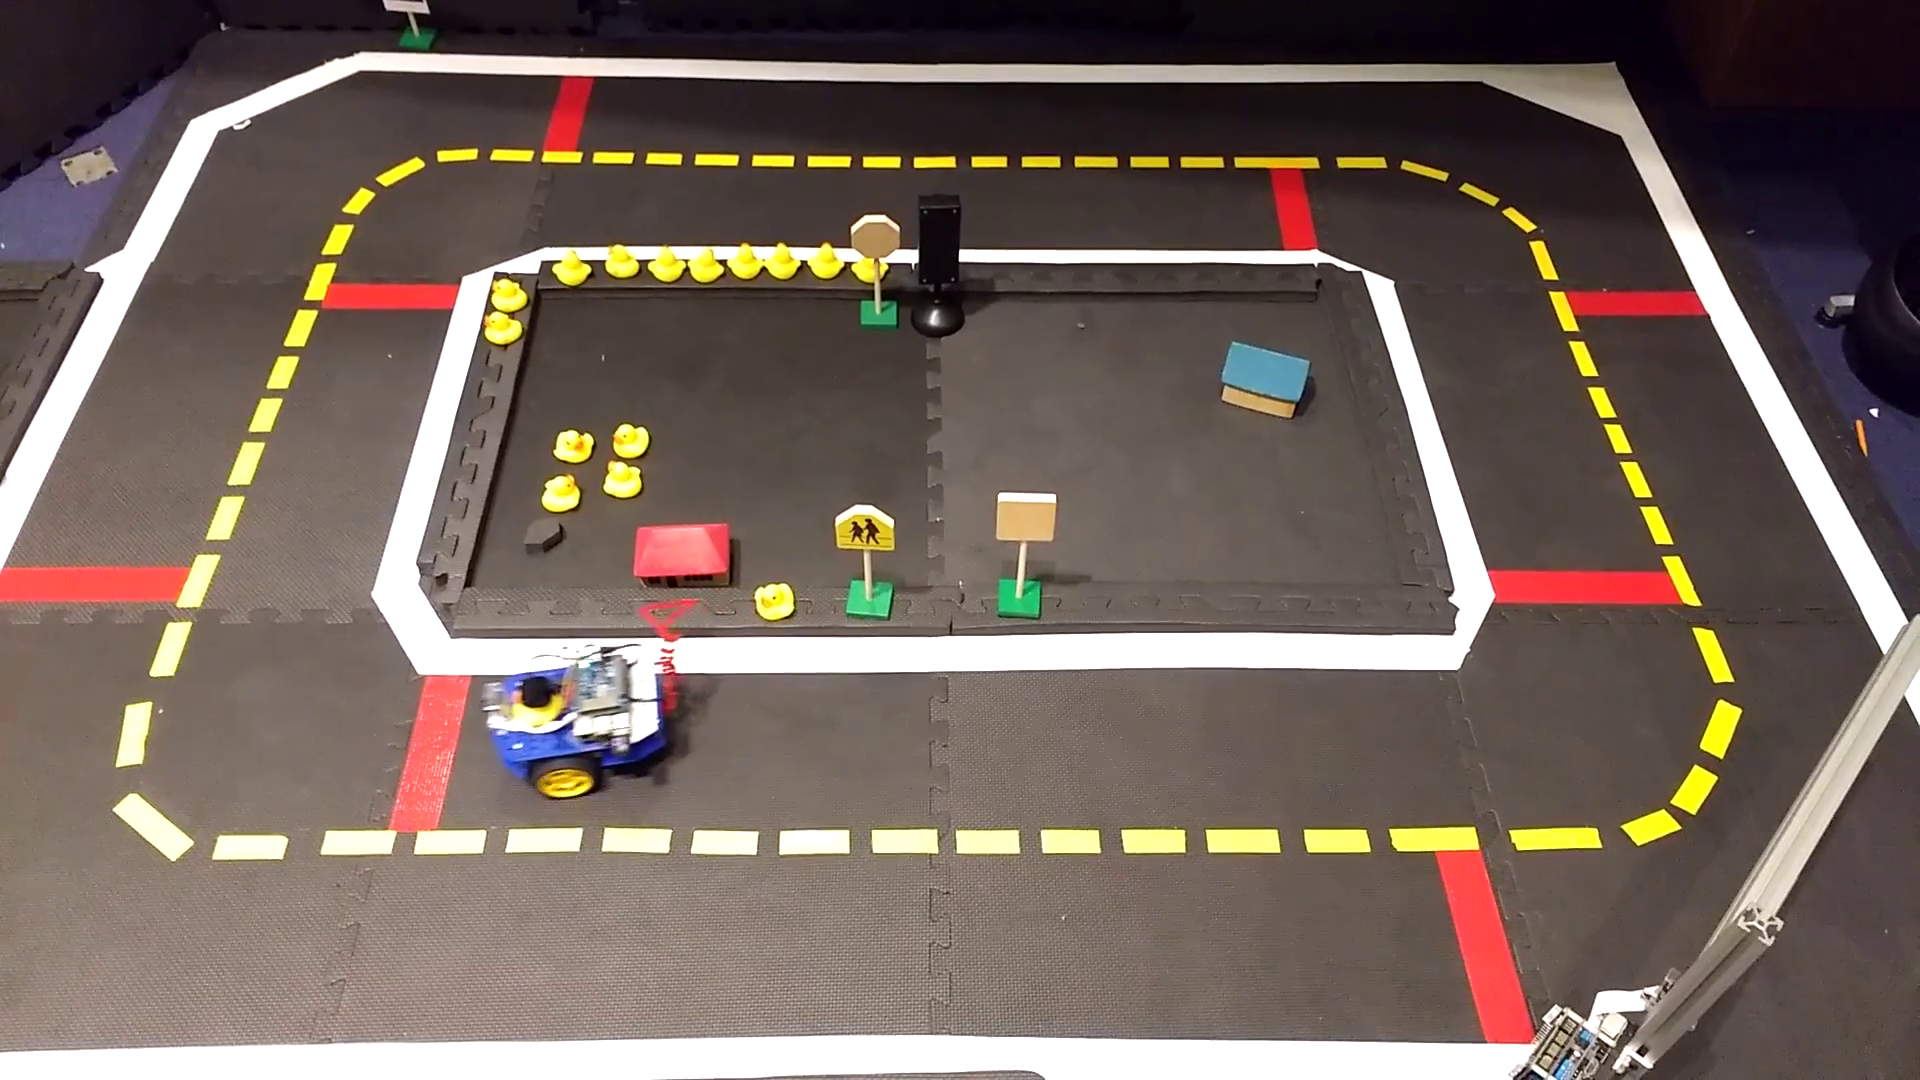
\includegraphics[width=1.0\textwidth,height=0.9\textheight,keepaspectratio]{videos/lane_following_loop.png}}{videos/lane_following_loop.mp4}
\end{center}
\end{frame}

%\begin{frame}{Videos}
%\begin{center}
%  \movie[showcontrols=true]{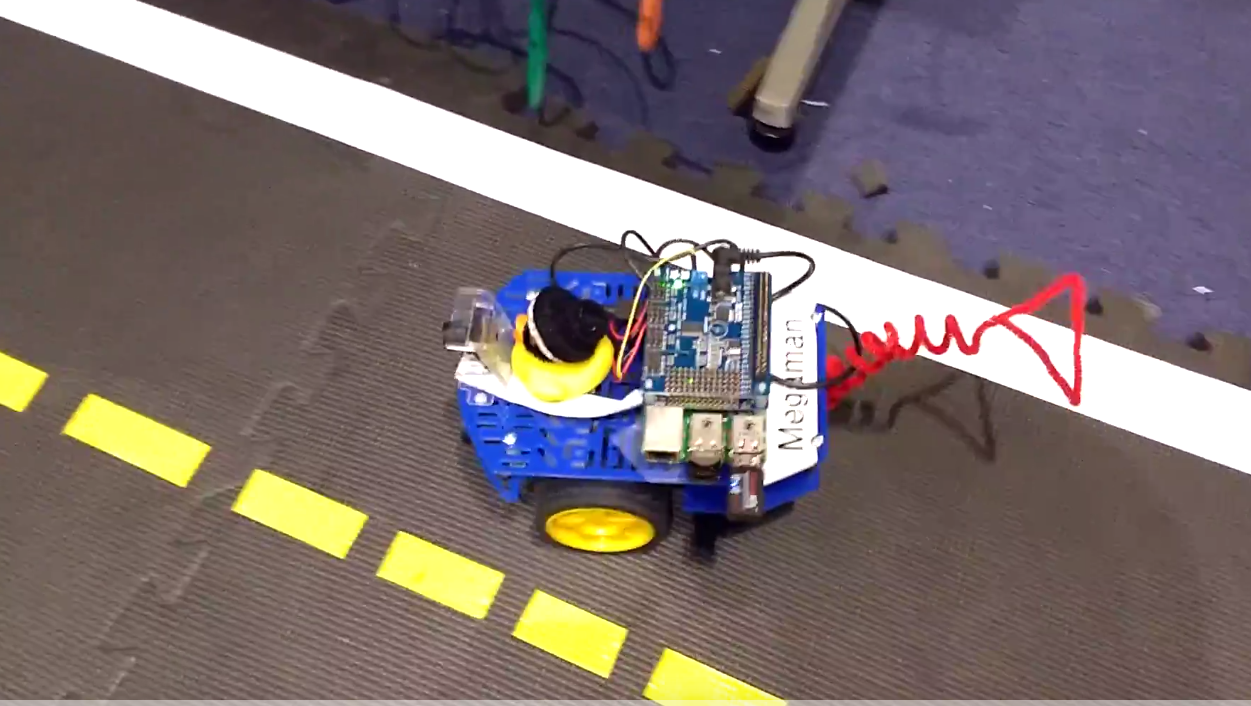
\includegraphics[width=0.8\textwidth]{videos/lane_following_2.png}}{videos/lane_following_2.mp4}
%\end{center}
%\end{frame}

\begin{frame}{Team Success}
\begin{columns}
	\begin{column}{0.55\textwidth}
		\begin{itemize}
			\item No man is an island
			\item \alert{Shih-Yuan} (glue)
\item Team members: Liam, Andrea, Hang, Steven, Changhyun, etc
		\end{itemize}
	\end{column}
	\begin{column}{0.45\textwidth}
		\centering
		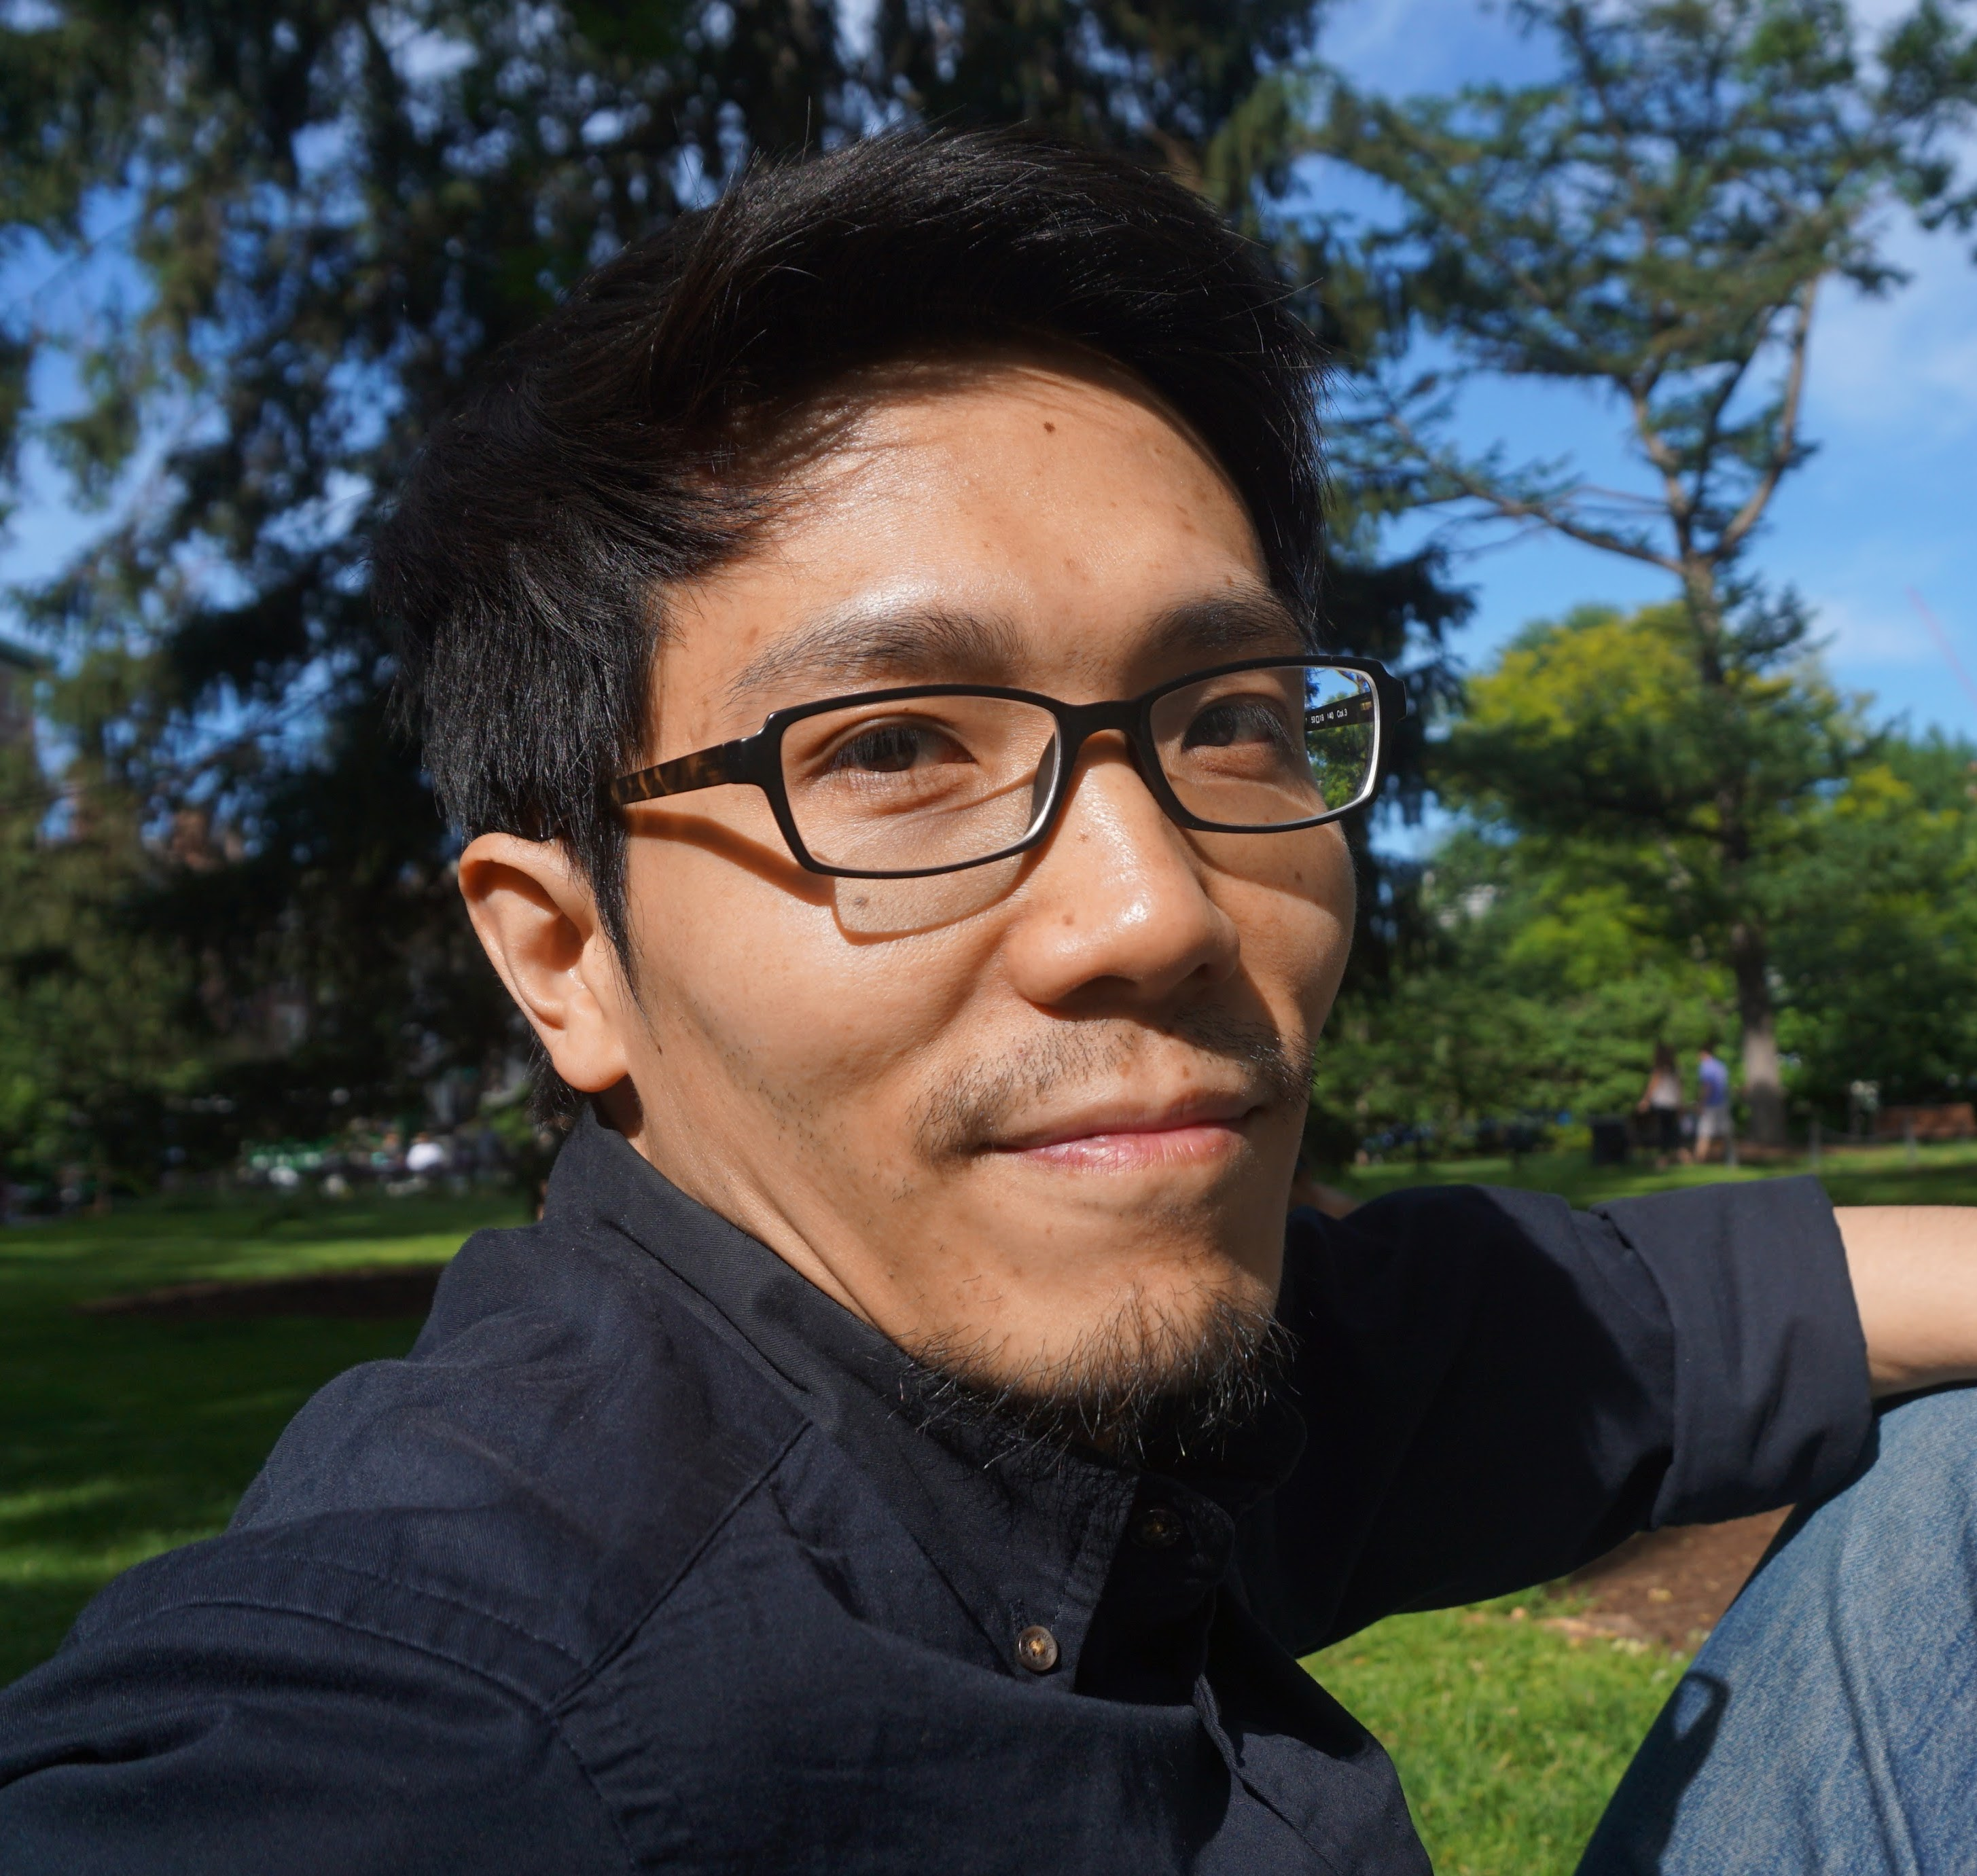
\includegraphics[width=0.6\textwidth]{fig/liu.jpg}
	\end{column}
\end{columns}

\end{frame}


\begin{frame}{Historical Note on Software for Robots}
\begin{columns}
	\begin{column}{0.55\textwidth}
%    \todo{Change figures}
		\begin{itemize}
			\item Want to advance state of the art
                        \item How parts talk to each other?
                        \item Build infrastructure
			\item Throw away 
		\end{itemize} 
        \end{column} 
        \begin{column}{0.45\textwidth} 
          \centering 
          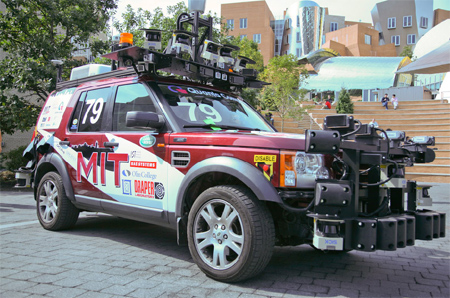
\includegraphics[width=\textwidth]{fig/urbanchallenge1.jpg} 
        \end{column}
\end{columns}

\end{frame}


\begin{frame}{What problems in software design?}
\begin{columns}
	\begin{column}{0.55\textwidth}
Thought process:
		\begin{itemize}
			\item One giant loop?
                        \item Many small pieces?
                        \item Reusable? 
		\end{itemize} 
        \end{column} 
        \begin{column}{0.45\textwidth} 
          \centering 
          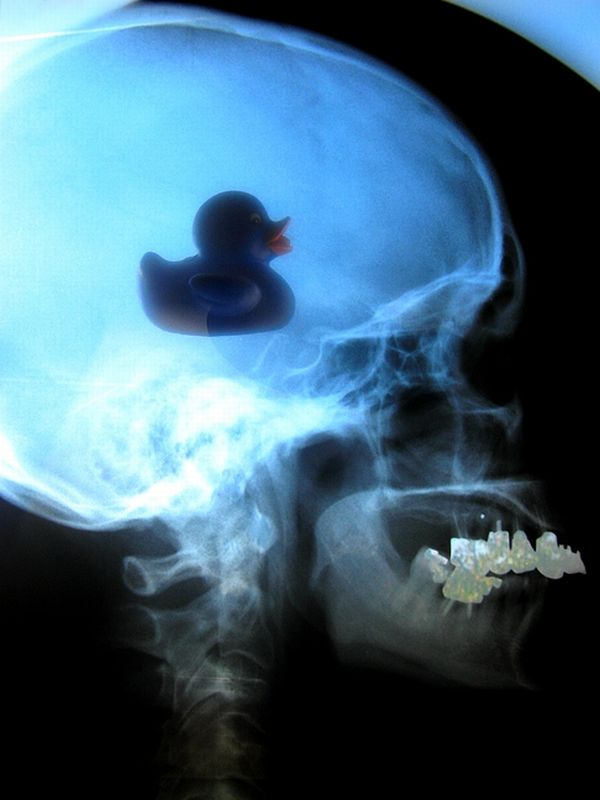
\includegraphics[width=0.6\textwidth]{fig/duckie-brain.jpg} 
        \end{column}
\end{columns}

\end{frame}



\begin{frame}[label=overview]{Overview}
	\tableofcontents
	%\tableofcontents[sectionstyle=show/shaded,subsectionstyle=show/shaded/shaded]
\end{frame}


\begin{frame}{Enter the Middleware}
%\todo{swap figure for OS, middleware, application}
%\todo{mention the glue}
%\todo{lives on a robot}
General Definition: software that connects software components. A layer that lies between the operating system and the applications on each side of a distributed computer network.
\begin{columns}
	\begin{column}{0.55\textwidth}
An abstraction:
		\begin{itemize}
			\item Not the operating system
                        \item Not the application
                        \item Right in the middle
		\end{itemize} 
        \end{column} 
        \begin{column}{0.45\textwidth} 
          \centering 
          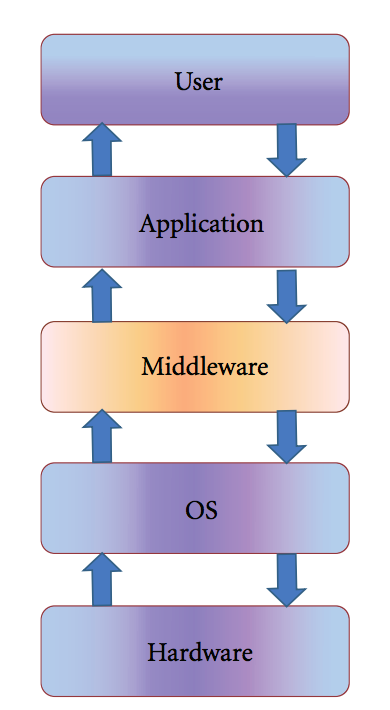
\includegraphics[width=0.4\textwidth]{fig/layers.png} 
          \centering 
          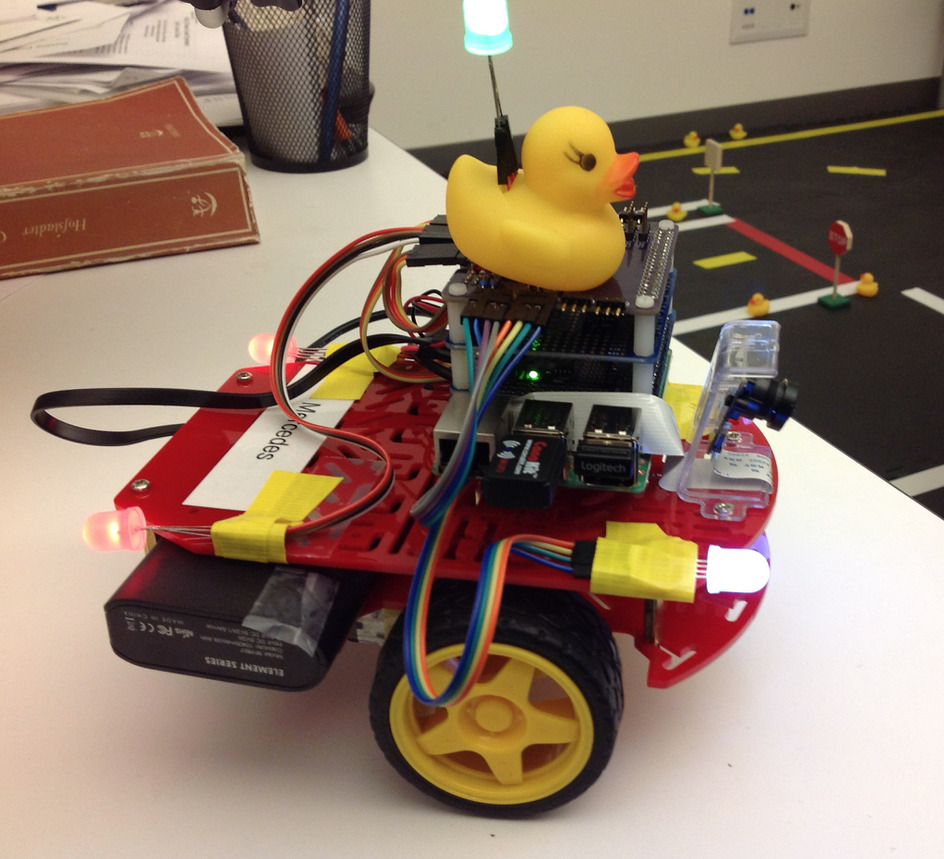
\includegraphics[width=0.4\textwidth]{fig/mercedes.jpg} 

        \end{column}
\end{columns}

\end{frame}



\begin{frame}{What do we gain?}
\begin{columns}
	\begin{column}{0.55\textwidth}
Every middleware must have:
		\begin{itemize}
			\item Abstraction from hardware
                          \item Hide communication
\end{itemize}

Good middlewares have:
\begin{itemize}
  \item Logging/Playback tools
                              \item Real-time analysis
\end{itemize}

Resulting benefits:
\begin{itemize}
                        \item Portable
                        \item Reusable
                        \item Saves time and money
		\end{itemize} 
        \end{column} 
        \begin{column}{0.45\textwidth} 
          \centering 
          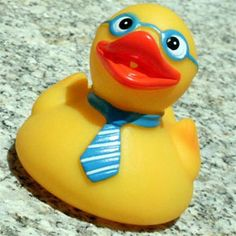
\includegraphics[width=0.6\textwidth]{fig/yay-duckie.jpg} 
        \end{column}
\end{columns}

\end{frame}

\begin{frame}{Many Robotics Middlewares!}
 \centering 
          
\includegraphics[width=0.3\textwidth]{fig/logo-ros.pdf}  \hspace{2cm}
\centering 
          
\includegraphics[width=0.1\textwidth]{fig/logo-MOOS.jpg}

\vspace

ROS, LCM, MOOS, JAUS, Orcos, Pyro, Player, Orca, Mira, OpenRTMaist, ASEBA, MARIE, RSCA, MRDS, OPROS, CLARAty, SmartSoft, ERSP, Webots, RoboFrame

\vspace

\centering 
          
\includegraphics[width=0.23\textwidth]{fig/logo-mira.png} \hspace{1.5cm}
\centering 
          
\includegraphics[width=0.3\textwidth]{fig/logo-openjaus.png}   
\end{frame}
 
\begin{frame}{Small Middleware Comparison}
%%\resizebox{10cm}{!}{
%\begin{tabular}{|l|l|l|l|}
%\hline \\
%  & ROS & LCM & MOOS \\ \hline
%Communication Structure & name-parameter server & decentralized & central database \\ \hline
%Communication Mechanism & intra-process, TCP, UDP  &  UDP multicast & TCP \\ \hline
%Data Transport          &  publisher / subscriber, RPC & publisher / subscriber & store / fetch \\ \hline
%Message Types           &  IDL using PODs  & IDL using PODs &  string, double \\ \hline
%Supported Languages     &  C++, Java, Python,... & C++ , Java, C#, Python, ... & C++, Java \\ \hline
%Supported Platforms     &  Linux, OS X and Win (partial) & Linux, Win, OS X & Linux, OS X
%\hline  
%\end{tabular}
\resizebox{12cm}{!}{
%\begin{center}
	\begin{tabular}{ |l|l|l|l| } 
		\hline
		& ROS & LCM & MOOS \\ \hline
		Communication Structure & name-/parameter server & decentralized & central database \\ \hline  
		Communication Mechanism & intra-process, TCP, UDP  &  UDP multicast & TCP \\ \hline
		Data Transport          &  publisher / subscriber, RPC & publisher / subscriber & store / fetch \\ \hline
		Message Types           &  IDL using PODs  & IDL using PODs &  string, double \\ \hline
		Supported Languages     &  C++, Java, Python,... & C++ , Java, C\#, Python, ... & C++, Java \\ \hline
		Supported Platforms     &  Linux, OS X (partial), and Win (partial) & Linux, Win, OS X & Linux, OS X \\
		\hline
	\end{tabular}
%\end{center}
}
\end{frame}

\begin{frame}{Intended Learning Outcome}
	\begin{block}{Learning Objectives}
		\begin{itemize}
			\item<1> Describe the value of middleware for robotics software development
			\item<0> Answer the question: ``What is your favorite robotics middleware and why is it ROS?''
			\item<0> Draw computation graph for simple robotic system using publish/subscribe model
			\item<0> Explain important ROS concepts such as node, topic, message, and parameters
			\item<0> Use important ROS command-line tools
			\item<0> Write a simple ROS node by following code examples
		\end{itemize}
	\end{block}
\end{frame}


\begin{frame}{Why ROS?}
\begin{columns}
	\begin{column}{0.55\textwidth}
		\begin{itemize}
			\item Communications infrastructure
                          \item Recording and playback of messages
                          \item Remote procedure calls
                          \item Distributed parameter system
                          \item Huge community
                          \item Sought after skills
                          \item Great for prototyping
		\end{itemize} 
        \end{column} 
        \begin{column}{0.45\textwidth} 
          \centering 
          
\includegraphics[width=0.6\textwidth]{fig/indigoigloo_600.png} 
        \end{column}
\end{columns}
\end{frame}

\begin{frame}{Which Tools?}
\begin{columns}
	\begin{column}{0.55\textwidth}
		\begin{itemize}
			\item command-line tools
                          \item graphical (rviz, rqt)              
		\end{itemize} 
        \end{column} 
        \begin{column}{0.45\textwidth} 
          \centering 
          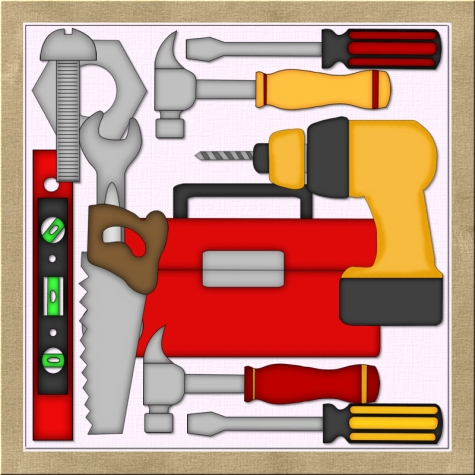
\includegraphics[width=0.6\textwidth]{fig/tools.jpeg} 
        \end{column}
\end{columns}
\end{frame}

\begin{frame}{Intended Learning Outcome}
	\begin{block}{Learning Objectives}
		\begin{itemize}
			\item<0> Describe the value of middleware for robotics software development
			\item<1> Answer the question: ``What is your favorite robotics middleware and why is it ROS?''
			\item<0> Draw computation graph for simple robotic system using publish/subscribe model
			\item<0> Explain important ROS concepts such as node, topic, message, and parameters
			\item<0> Use important ROS command-line tools
			\item<0> Write a simple ROS node by following code examples
		\end{itemize}
	\end{block}
\end{frame}


\section{Architecture Overview}
\begin{frame}[label=overview]{Overview}
%	\tableofcontents
	\tableofcontents[sectionstyle=show/shaded,subsectionstyle=show/shaded/shaded]
\end{frame}

\begin{frame}{Meet the Team: Shih-Yuan Liu}
	\begin{block}{How to pronounce my name?}<1->
		sh-U-when
	\end{block}
	\begin{block}{Where am I from?}<2->
		\begin{itemize}
			\item Taiwan
			\item U.C. Berkeley
		\end{itemize}
	\end{block}
	\begin{block}{What am I doing here at MIT?}<3->
		\begin{itemize}
			\item Postdoc with Prof. Jonathan How (Aerospace Controls Lab)
			\item Control and Planning for Autonomous Vehicles
		\end{itemize}
	\end{block}
	\begin{block}{What am I doing here in Duckietown?}<4->
		\begin{itemize}
			\item ROS Man
			\item Control
		\end{itemize}
	\end{block}
\end{frame}

%\begin{frame}{Intended Learning Outcome}
%	\begin{block}{Learning Objectives}
%	\begin{itemize}[<+->]
%		\item Draw computation graph for simple robotic system using publish/subscribe model
%		\item Describe the value of middleware for robotics software development
%		\item Explain important ROS concepts such as node, topic, message, and parameters
%		\item Use important ROS command-line tools
%		\item Answer the question: ``What is your favorite robotics middleware and why is it ROS?''
%		\item Write a simple ROS node by following code examples
%	\end{itemize}
%	\end{block}
%\end{frame}

\begin{frame}{Behind the Curtain Look at Lane Following}
	\begin{center}
		\movie[showcontrols=false]{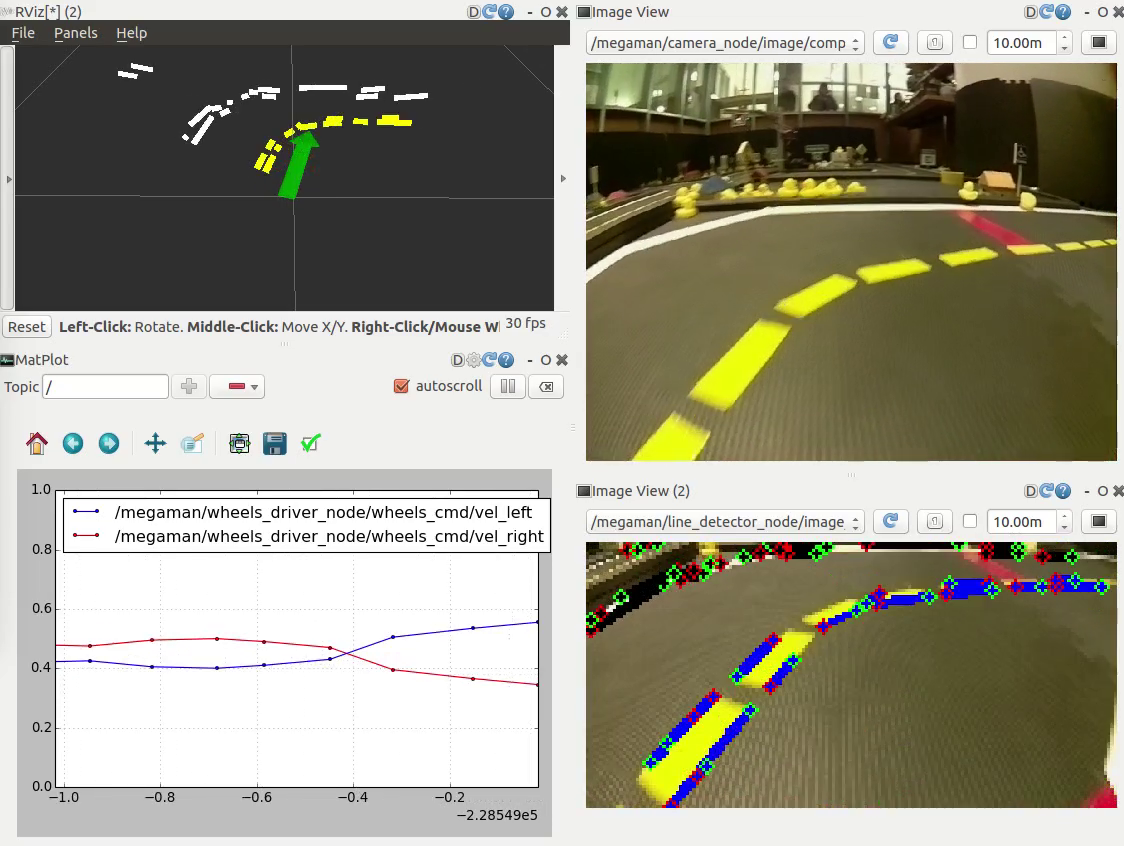
\includegraphics[width=\textwidth,height=0.85\textheight,keepaspectratio]{videos/lane_following_all.png}}{videos/lane_following_all.mp4}
	\end{center}
\end{frame}


\begin{frame}{Computation Graph: Publish/Subscribe}
	\begin{columns}[T]
		\begin{column}{0.5\textwidth}
			\begin{overlayarea}{\textwidth}{\textheight}
			\centering
%			\only<1>{\includedot[width=\textwidth,height=0.8\textheight,keepaspectratio]{dot/robot_as_graph_1}}%
			\only<1>{\includedot[width=\textwidth,height=0.8\textheight,keepaspectratio]{dot/robot_as_graph_2}}%
			\only<2>{\includedot[width=\textwidth,height=0.8\textheight,keepaspectratio]{dot/robot_as_graph_2a}}%
			\only<3>{\includedot[width=\textwidth,height=0.8\textheight,keepaspectratio]{dot/robot_as_graph_3}}%
			\only<4>{\includedot[width=\textwidth,height=0.8\textheight,keepaspectratio]{dot/robot_as_graph_4}}%
			\only<5>{\includedot[width=\textwidth,height=0.8\textheight,keepaspectratio]{dot/robot_as_graph_5}}%
			\end{overlayarea}
		\end{column}
		\begin{column}{0.5\textwidth}
			\only<1-2>{
			\begin{figure}
				\centering
				\begin{subfigure}
					\centering
					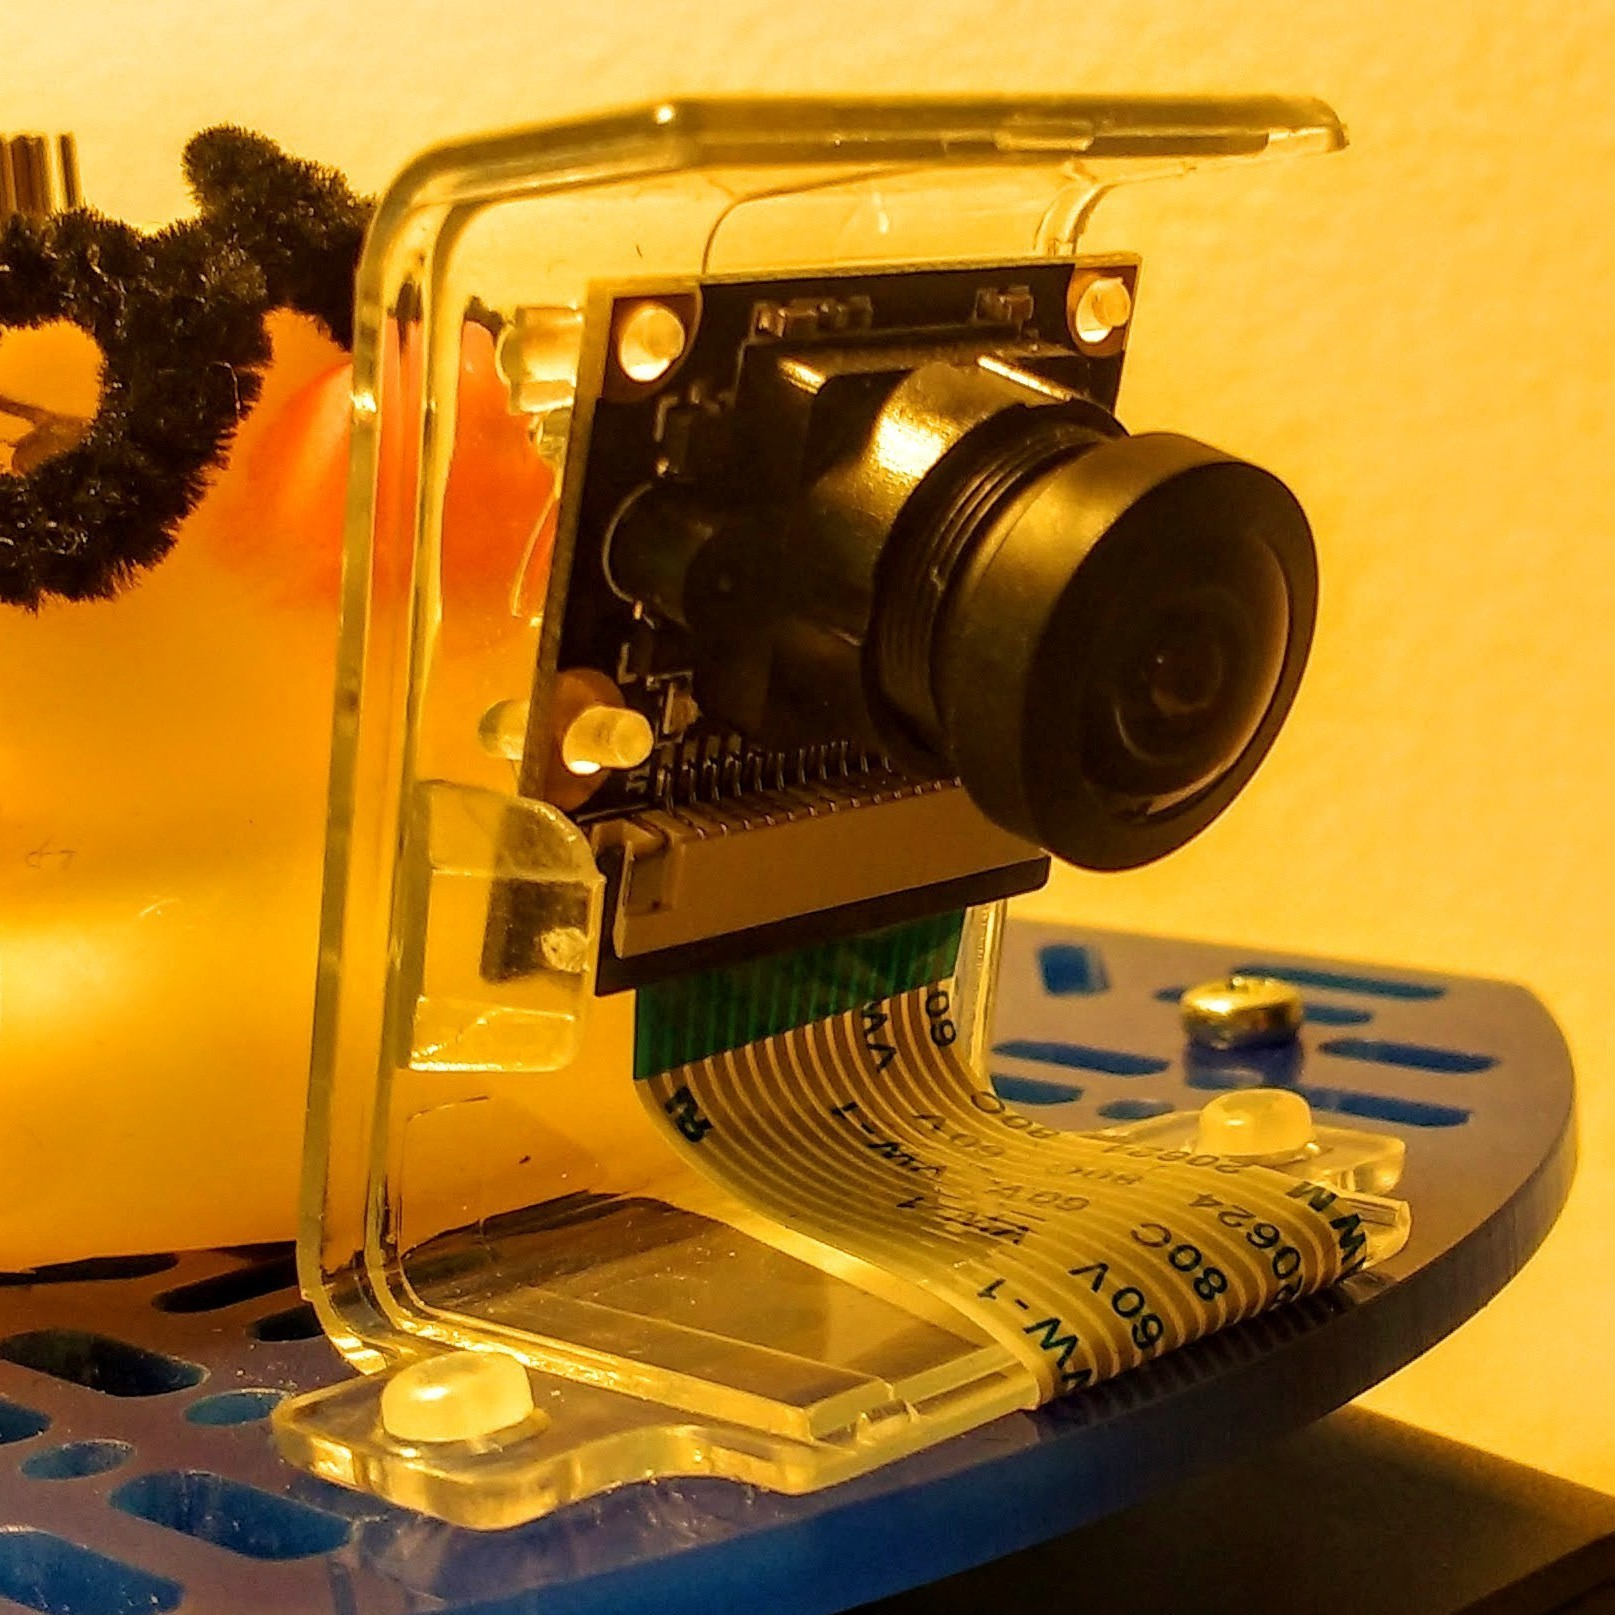
\includegraphics[width=\textwidth,height=0.3\textheight,keepaspectratio]{dot/camera.jpg}\\
					Sensors: Camera\vspace{10pt}
				\end{subfigure}
				
				\begin{subfigure}
					\centering
					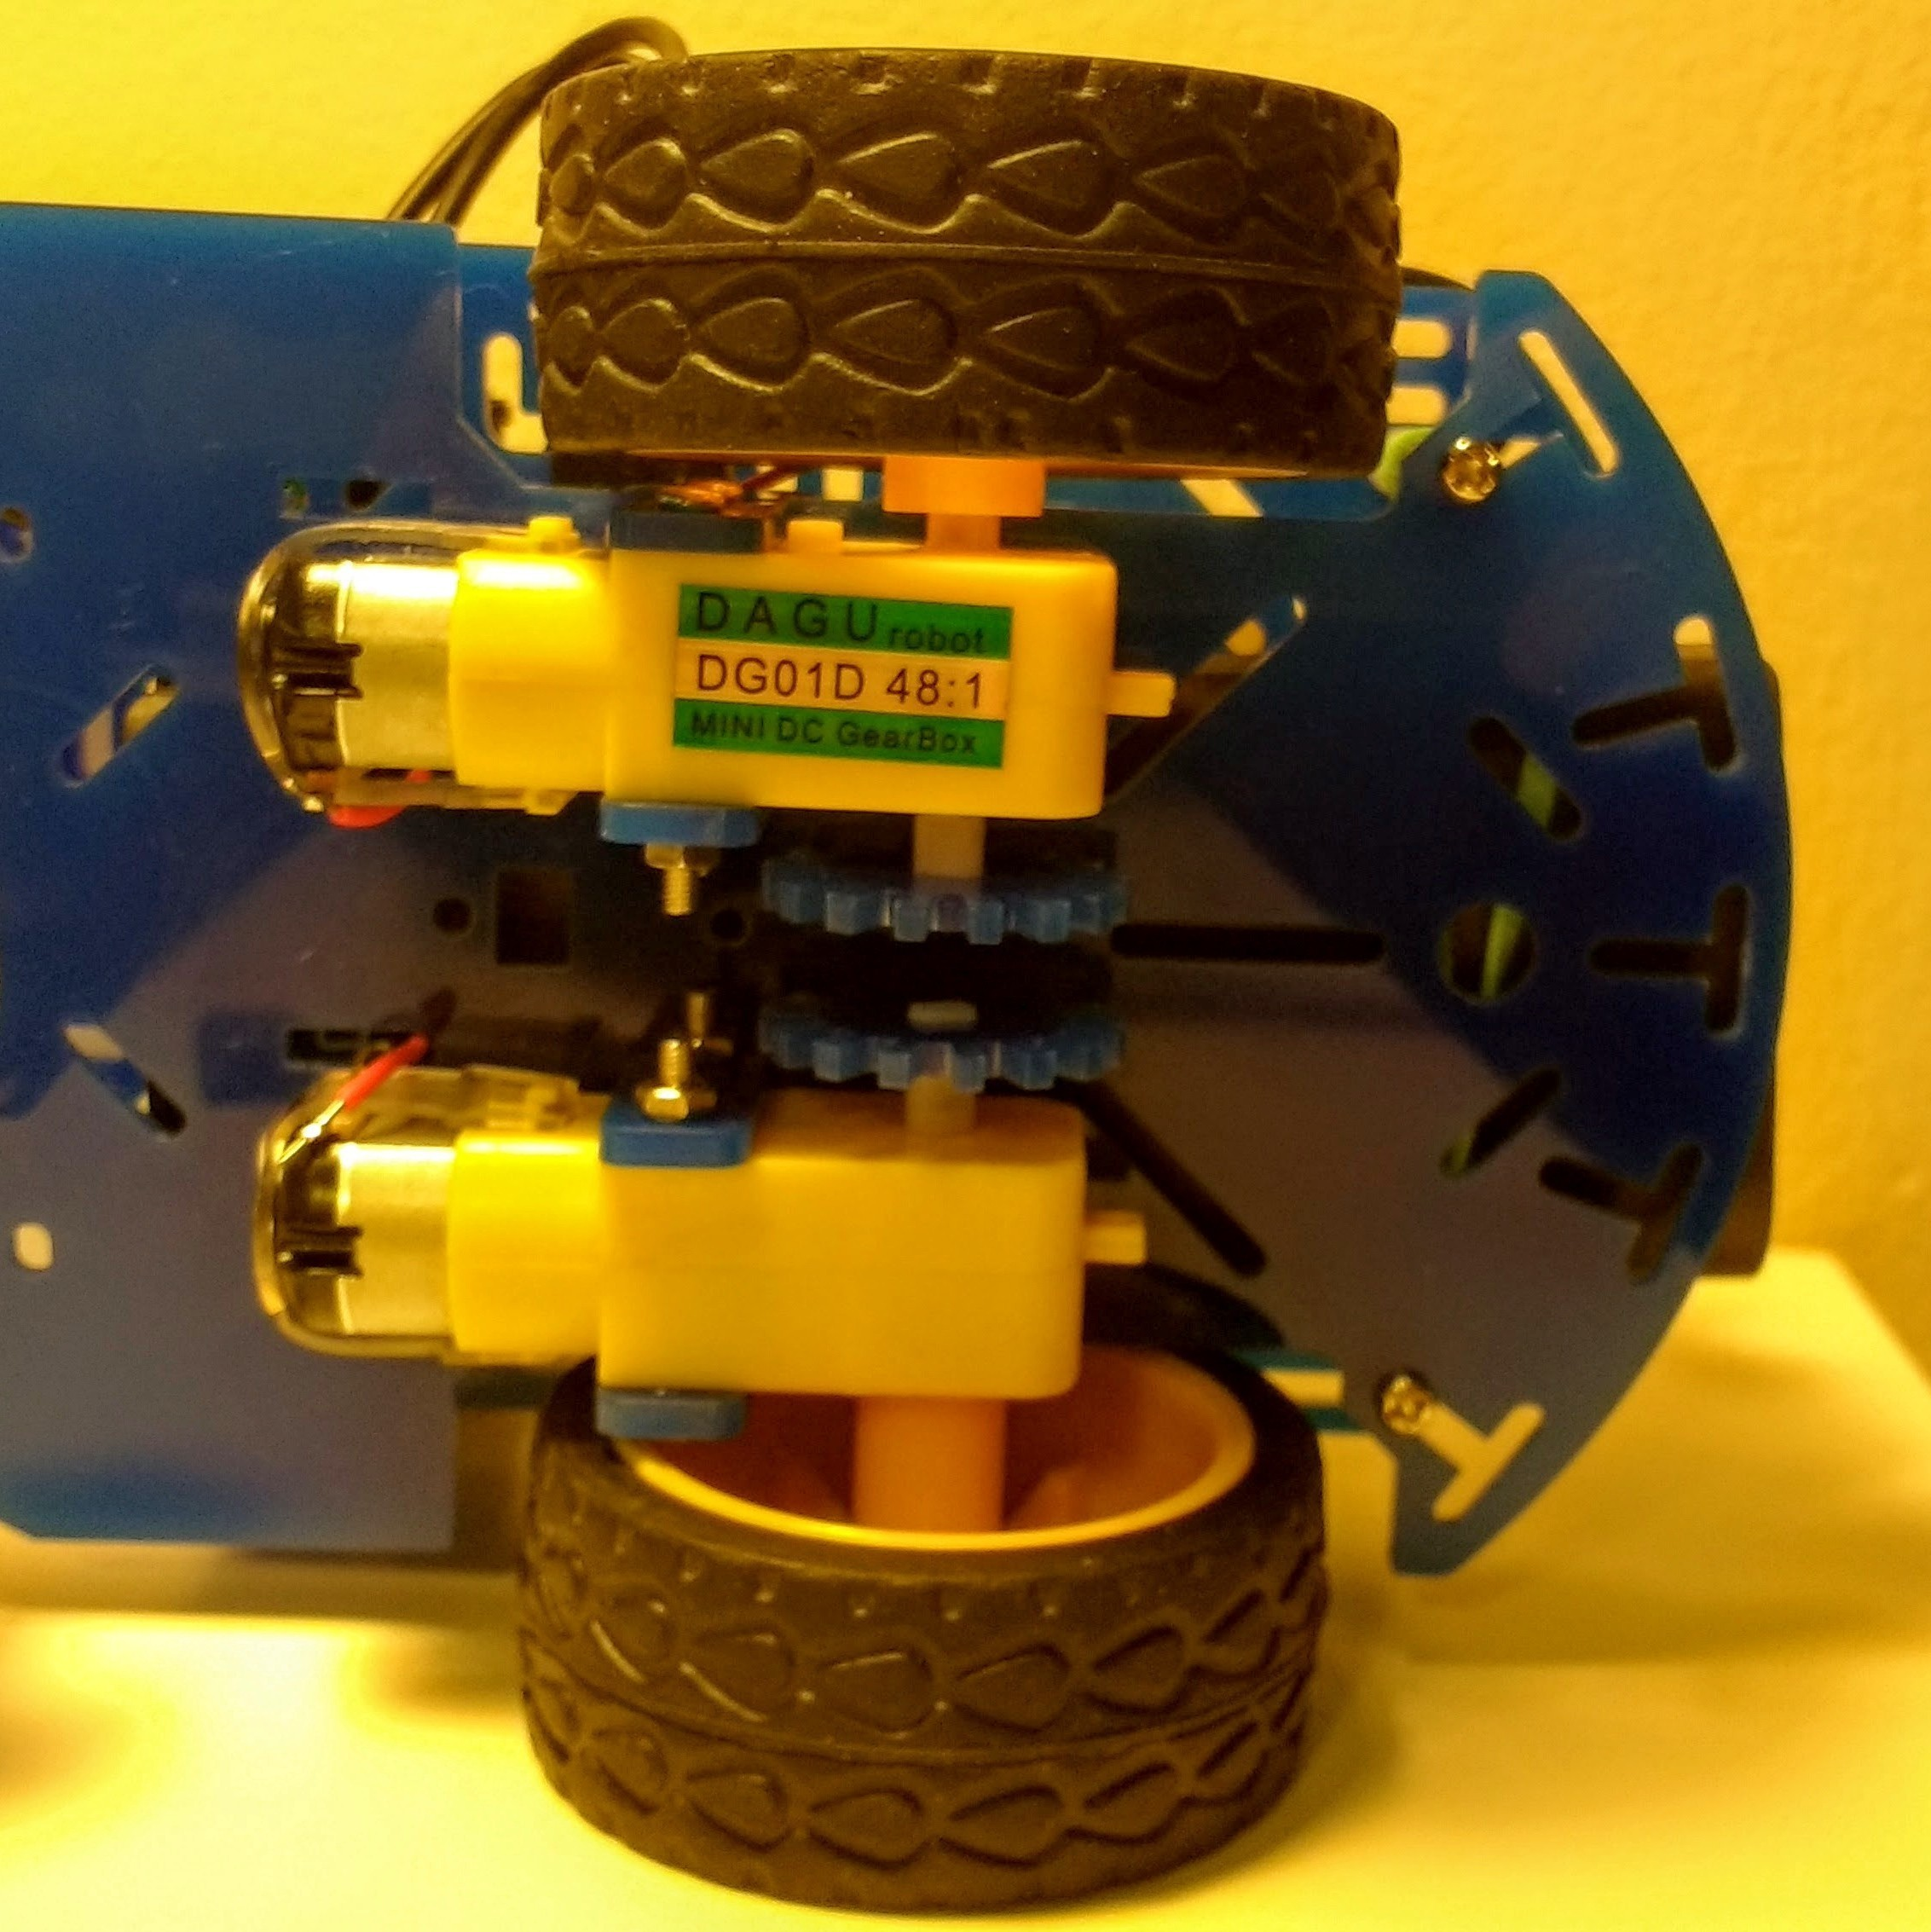
\includegraphics[width=\textwidth,height=0.3\textheight,keepaspectratio]{dot/wheels.jpg}\\
					Actuators: Wheel Motors
				\end{subfigure}
			\end{figure}
			}
			\only<3->{
				\centering
				\movie[showcontrols=false]{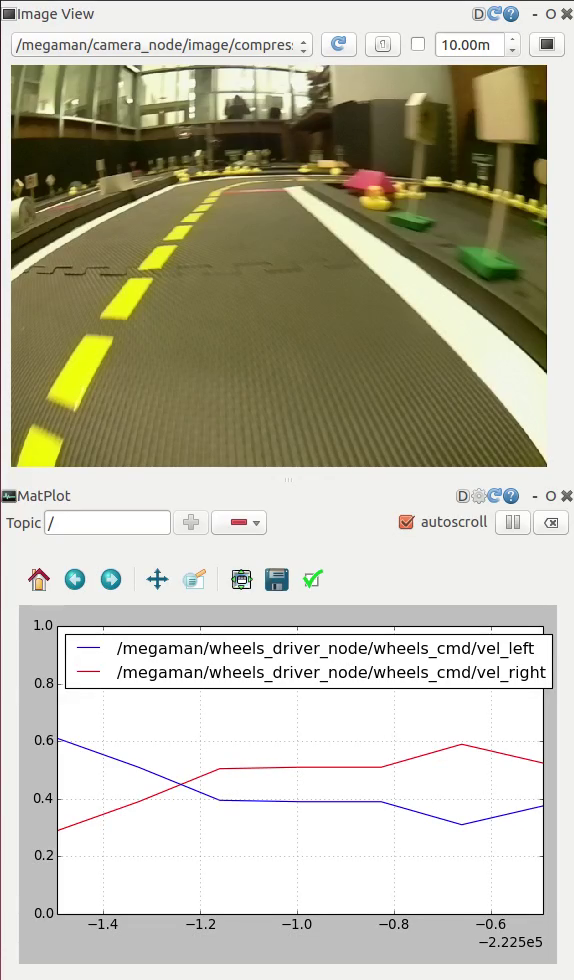
\includegraphics[width=\textwidth,height=0.8\textheight,keepaspectratio]{videos/lane_control_IO.png}}{videos/lane_control_IO.mp4}
				}
		\end{column}
	\end{columns}
\end{frame}

\begin{frame}{Example: Lane Following}
\begin{center}
\includedot[width=\textwidth,height=0.8\textheight,keepaspectratio]{dot/lane_following}%
\end{center}
\end{frame}

\begin{frame}{Line Detector}
\framesubtitle{Hang Zhao}
	\begin{columns}
		\begin{column}{0.6\textwidth}
			\centering
			\only<1>{\includedot[width=\textwidth,height=0.8\textheight,keepaspectratio]{dot/lane_following_line_detection}}%
			\only<2>{\includedot[width=\textwidth,height=0.8\textheight,keepaspectratio]{dot/lane_following_line_detection_zoom}}%
		\end{column}
		\begin{column}{0.4\textwidth}
		  \movie[showcontrols=false]{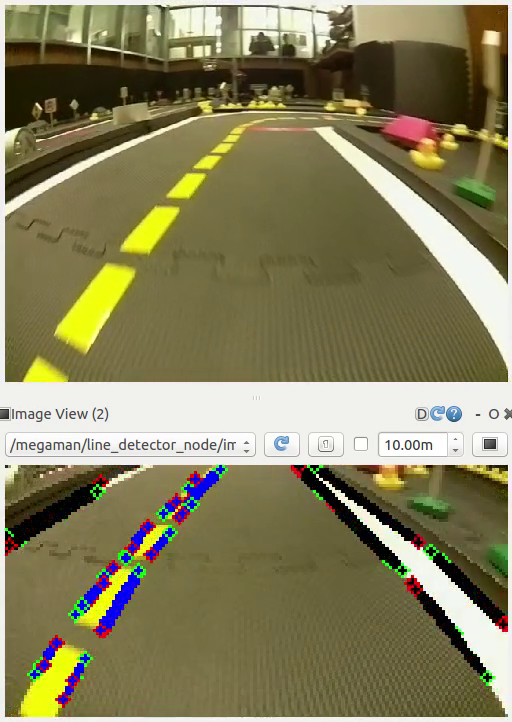
\includegraphics[width=\textwidth,height=0.8\textheight,keepaspectratio]{videos/line_detection.png}}{videos/line_detection.mp4}
		\end{column}
	\end{columns}
\end{frame}

\begin{frame}{Ground Projector}
\framesubtitle{Dr. Changhyun Choi}
	\begin{columns}
		\begin{column}{0.6\textwidth}
			\centering
			\only<1>{\includedot[width=\textwidth,height=0.8\textheight,keepaspectratio]{dot/lane_following_ground_projection}}%
			\only<2>{\includedot[width=\textwidth,height=0.8\textheight,keepaspectratio]{dot/lane_following_ground_projection_zoom}}%
		\end{column}
		\begin{column}{0.4\textwidth}
		  \movie[showcontrols=false]{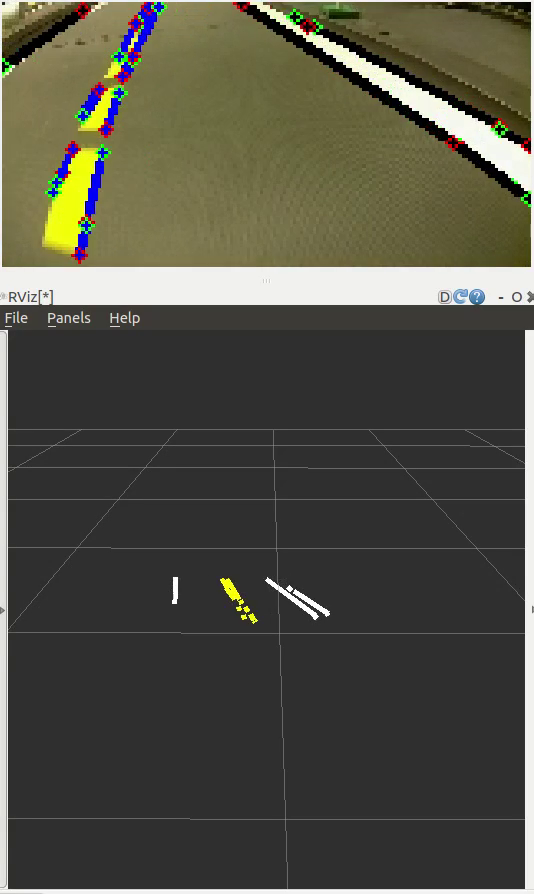
\includegraphics[width=\textwidth,height=0.8\textheight,keepaspectratio]{videos/ground_projection.png}}{videos/ground_projection.mp4}
		\end{column}
	\end{columns}
\end{frame}

\begin{frame}{Lane Filter Node}
\framesubtitle{Dr. Liam Paull}
	\begin{columns}
		\begin{column}{0.6\textwidth}
			\centering
			\only<1>{\includedot[width=\textwidth,height=0.8\textheight,keepaspectratio]{dot/lane_following_lane_filter}}%
			\only<2>{\includedot[width=\textwidth,height=0.8\textheight,keepaspectratio]{dot/lane_following_lane_filter_zoom}}%
		\end{column}
		\begin{column}{0.4\textwidth}
		  \movie[showcontrols=false]{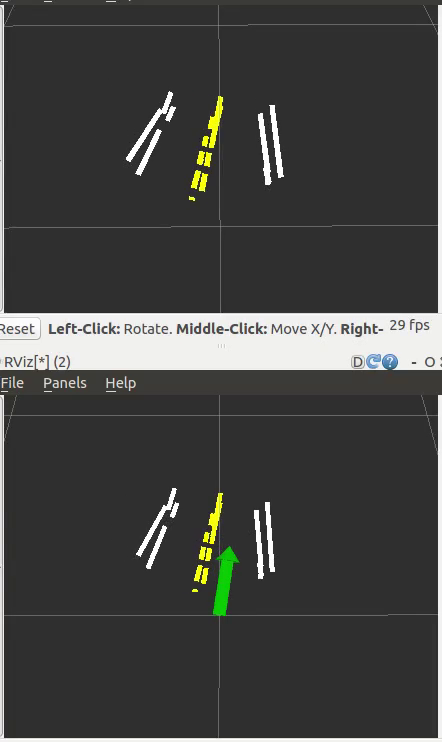
\includegraphics[width=\textwidth,height=0.8\textheight,keepaspectratio]{videos/lane_filter.png}}{videos/lane_filter.mp4}
		\end{column}
	\end{columns}
\end{frame}

\begin{frame}{Lane Controller}
\framesubtitle{Steven Chen}
	\begin{columns}
		\begin{column}{0.6\textwidth}
			\centering
			\only<1>{\includedot[width=\textwidth,height=0.8\textheight,keepaspectratio]{dot/lane_following_lane_control}}%
			\only<2>{\includedot[width=\textwidth,height=0.8\textheight,keepaspectratio]{dot/lane_following_lane_control_zoom}}%
		\end{column}
		\begin{column}{0.4\textwidth}
		  \movie[showcontrols=false]{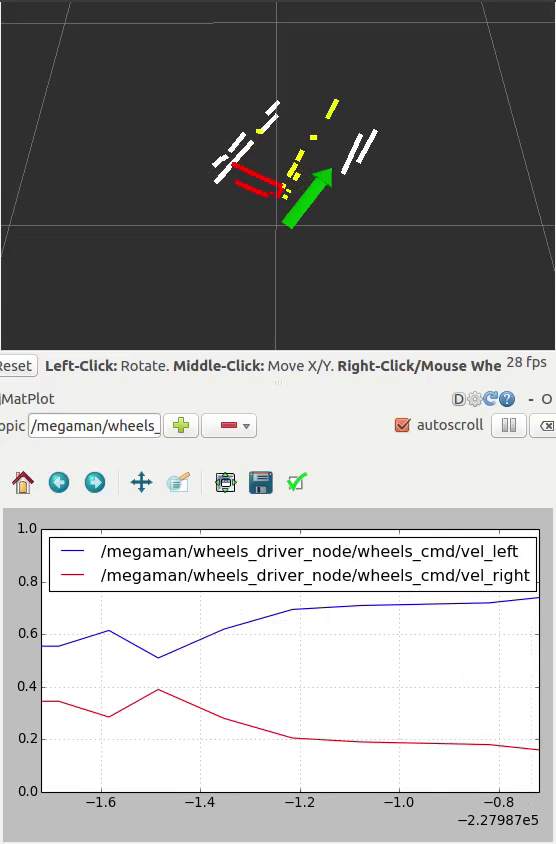
\includegraphics[width=\textwidth,height=0.8\textheight,keepaspectratio]{videos/lane_control.png}}{videos/lane_control.mp4}
		\end{column}
	\end{columns}
\end{frame}

\begin{frame}{Lane Folloiwng Summary}
	\begin{center}
		\movie[showcontrols=false]{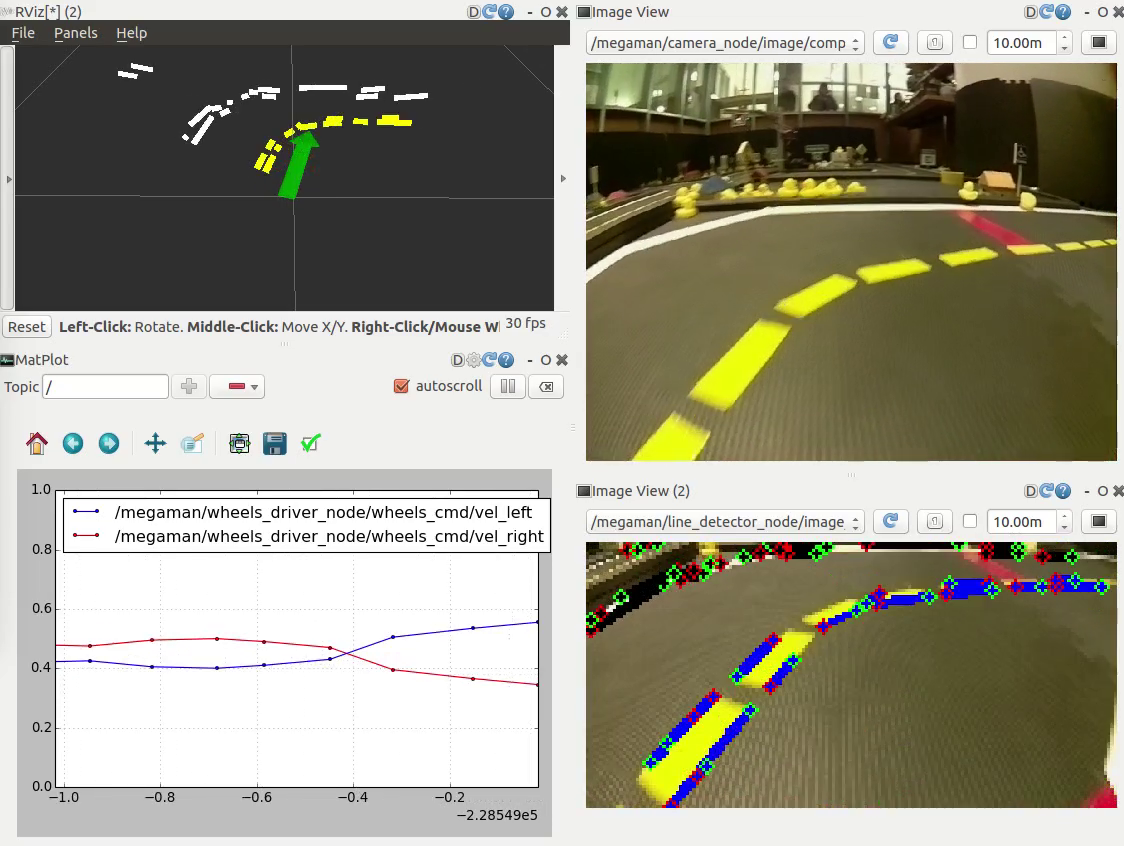
\includegraphics[width=\textwidth,height=0.85\textheight,keepaspectratio]{videos/lane_following_all.png}}{videos/lane_following_all.mp4}
	\end{center}
\end{frame}

\begin{frame}{Intended Learning Outcome}
	\begin{block}{Learning Objectives}
		\begin{itemize}
			\item<0> Describe the value of middleware for robotics software development
			\item<0> Answer the question: ``What is your favorite robotics middleware and why is it ROS?''
			\item<1> Draw computation graph for simple robotic system using publish/subscribe model
			\item<0> Explain important ROS concepts such as node, topic, message, and parameters
			\item<0> Use important ROS command-line tools
			\item<0> Write a simple ROS node by following code examples
		\end{itemize}
	\end{block}
\end{frame}
 
\begin{frame}{Why do we need this?}
\framesubtitle{Duckietown Architecture}
\begin{center}
	\includedot[width=\textwidth,height=0.8\textheight,keepaspectratio]{dot/Duckietown_ROS_Diagram}%
\end{center}
\end{frame}

\begin{frame}{Intended Learning Outcome}
	\begin{block}{Learning Objectives}
		\begin{itemize}
			\item<1> Describe the value of middleware for robotics software development
			\item<0> Answer the question: ``What is your favorite robotics middleware and why is it ROS?''
			\item<0> Draw computation graph for simple robotic system using publish/subscribe model
			\item<0> Explain important ROS concepts such as node, topic, message, and parameters
			\item<0> Use important ROS command-line tools
			\item<0> Write a simple ROS node by following code examples
		\end{itemize}
	\end{block}
\end{frame}

\section{ROS Concept Overview}
\begin{frame}[label=overview]{Overview}
%	\tableofcontents
	\tableofcontents[sectionstyle=show/shaded,subsectionstyle=show/shaded/shaded]
\end{frame}


\begin{frame}{Nodes and Topics}
	\begin{columns}[c]
		\begin{column}{0.5\textwidth}
			%\todo[inline]{Graph. What is a node? Node/Edge explaination.}
			%\todo[inline]{Topic example with images. command plots etc.}
			\begin{itemize}[<+->]
				\item Nodes:
					\begin{itemize}
					\item Executables (\texttt{python} or \texttt{C++})
					\item Each node is a process
					\item Publishes/Subscribes to Topics
					\end{itemize}
				\item Topics:
					\begin{itemize}
					\item Passes information between nodes
					\item Topic type defined by messages
					\item Support many-to-many communication
					\end{itemize}
			\end{itemize}
		\end{column}
		\begin{column}{0.5\textwidth}
			% \centering
			\includedot[width=\textwidth,height=0.8\textheight,keepaspectratio]{dot/node_and_topic}
%			\todo[inline]{Add two way communication figure}
%			\todo[inline]{Oval and Square are inversed on the diagram.... Fix this.}
		\end{column}
	\end{columns}
\end{frame}

\begin{frame}{ROS Master}
	\framesubtitle{The Telephone Operator}
	\begin{columns}[T]
		\begin{column}{0.6\textwidth}
%			\todo[inline]{Transparnet on which machine running which code.}
			\begin{itemize}
			\item<1-> Handles communication between nodes
			\item<2-> Connects publisher and subscriber through topics
			\item<3-> Traffic does \alert{not} go through the master once connected
			\item<4-> TCP/IP connection
			\end{itemize}
		\end{column}
		\begin{column}{0.4\textwidth}
			\centering
			\includegraphics[width=\textwidth]{fig/tele_operator.jpg}
		\end{column}
	\end{columns}
%  \todo{Consider more specific examples?}
%  \todo{Specify machines}
	\only<1-4>{\includedot[width=\textwidth,height=\textheight,keepaspectratio]{dot/master_1}}
	\only<5>{\includedot[width=\textwidth,height=\textheight,keepaspectratio]{dot/master_2}}
	\only<6>{\includedot[width=\textwidth,height=\textheight,keepaspectratio]{dot/master_3}}
	\only<7>{\includedot[width=\textwidth,height=\textheight,keepaspectratio]{dot/master_4}}
	\only<8>{\includedot[width=\textwidth,height=\textheight,keepaspectratio]{dot/master_5}}
\end{frame}

\begin{frame}{Commandline Tools and Demo}
	\begin{columns}
		\begin{column}{0.5\textwidth}
			\begin{itemize}
				\item Start a ROS Master:\\\inline{roscore}
				\item Launch a launch file:\\\inline{roslaunch pkg_name launch_file}
				\item View communication graph:\\\inline{rqt_graph}
				\item List all nodes:\\\inline{rosnode list}
				\item Info of a node:\\\inline{rosnode info node_name}
			\end{itemize}
		\end{column}
		\begin{column}{0.5\textwidth}
			\centering
			Live demo
%			\todo[inline]{Terminals are scary}
%			\todo[inline]{Package are not introduced.}
%			\todo[inline]{Use camera and rqt graph as an example}
%			\todo[inline]{rostopic hz}
		\end{column}
	\end{columns}
\end{frame}

\begin{frame}{Commandline Tools and Demo}
	\begin{columns}
		\begin{column}{0.5\textwidth}
			\begin{itemize}
				\item List all topics:\\\inline{rostopic list}
				\item Info of a topic:\\\inline{rostopic info topic_name}
				\item Listen to a topic:\\\inline{rostopic echo topic_name}
				\item Check frequency of a topic:\\\inline{rostopic hz topic_name}
				\item Plot a topic:\\\inline{rqt_plot}
				\item 3D Visualizer:\\\inline{rviz}
			\end{itemize}
		\end{column}
		\begin{column}{0.5\textwidth}
			\centering
			Live demo
			%			\todo[inline]{Terminals are scary}
			%			\todo[inline]{Package are not introduced.}
			%			\todo[inline]{Use camera and rqt graph as an example}
			%			\todo[inline]{rostopic hz}
		\end{column}
	\end{columns}
\end{frame}


\begin{frame}{Messages}
	\begin{columns}
		\begin{column}{1.0\textwidth}
			\begin{itemize}[<+->]
				\item The content and structure of a topic is defined by a message
				\item Application Programming Interface (API) for nodes
				\item Defined in \inline{.msg} files
				\item Primitive Type: \inline{bool}, \inline{string}, \inline{float32}, \inline{int32}, ... etc
				\begin{itemize}
					\item Single value field: \inline{field_type field_name}\\%
					\item Fixed-length field: \inline{field_type[n] field_name}\\%
					\item Variable-length field: \inline{field_type[] field_name}
				\end{itemize}
			\end{itemize}
		\end{column}
%		\begin{column}{0.3\textwidth}
%			\centering
%			%\includegraphics[width=\textwidth]{}
%		\end{column}
	\end{columns}
\end{frame}

\begin{frame}{Commandline Tools and Demo}
	\begin{columns}
		\begin{column}{0.6\textwidth}
			\begin{itemize}
				\item Look up definition of a message:\\\inline{rosmsg show pkg_name msg_name}
				\item Common message packages:
					\begin{itemize}
						\item \inline{std_msgs}
						\item \inline{geometry_msgs}
						\item \inline{sensor_msgs}
						\item \inline{duckietown_msgs}
					\end{itemize}
			\end{itemize}
		\end{column}
		\begin{column}{0.4\textwidth}
			\centering
			Live Demo
		\end{column}
	\end{columns}
\end{frame}

\begin{frame}{Parameters}
	\begin{columns}
		\begin{column}{1.0\textwidth}
			\begin{itemize}[<+->]
				\item Publish/Subscribe does not suit everything
				\item Nodes often requires parameterization
					\begin{itemize}
						\item Camera resolution
						\item Threshold
						\item Controller gain
					\end{itemize}
				\item Kept on the parameter server:
					\begin{itemize}
						\item Initialized with master
						\item Parameters persist until master is killed
					\end{itemize}
				\item Can be set and changed at run time
			\end{itemize}
		\end{column}
	\end{columns}
\end{frame}

\begin{frame}{Commandline Tools and Demo for Parameters}
	\begin{columns}
		\begin{column}{0.5\textwidth}
			\begin{itemize}
				\item List parameters:\\\inline{rosparam list}
				\item Get parameter:\\\inline{rosparam get param_name}
				\item Set parameter:\\\inline{rosparam set param_name}
				\item Dump parameters into file:\\\inline{rosparam dump file_name [namespace]}
				\item Read parameters from file:\\\inline{rosparam load file_name [namespace]}
			\end{itemize}
		\end{column}
		\begin{column}{0.5\textwidth}
			\centering
      Live Demo
		\end{column}
	\end{columns}
\end{frame}

%\begin{frame}{Services}
%	TODO
%\end{frame}

\begin{frame}{Launch File}
	\begin{itemize}
		\item XML format file can specify almost all aspects/actions of ROS
		\begin{itemize}
			\item Launch nodes, set/load parameters, remap topics, include other launch files, pass commandline arguments
		\end{itemize}
		\item Syntax: \inputminted{xml}{snippet/launch_syntax.launch}
		\item Tags:
			\begin{itemize}
				\item \inline{<launch>}: Container of launch files.
				\item \inline{<group>}: Group nodes together.
				\item \inline{<arg>}: I/O of launch files.
				\item \inline{<node>}: Run a node.
				\item \inline{<include>}: Invoke other launch files.
			\end{itemize}
	\end{itemize}
\end{frame}

\begin{frame}{Attribute and Elements for \texttt{<node>}}
	\begin{columns}
		\begin{column}{0.7\textwidth}
			\begin{itemize}
				\item Key attributes:
					\begin{itemize}
						\item \inline{pkg}: Name of package
						\item \inline{type}: Executable file name
						\item \inline{name}: Name of the node
						\item \inline{args}: Commandline arguments for the exec
						\item \inline{machine}: Machine to run the node
						\item \inline{ns}: Namespace of the node
						\item \inline{output}: Outputs of the node
						\item \inline{if/unless}: Conditional
					\end{itemize}
				\item Key elements:
					\begin{itemize}
						\item \inline{<remap>}: Remap topics
						\item \inline{<rosparam>}: Set parameters
						\item \inline{<param>}: Set parameters
					\end{itemize}
			\end{itemize}
		\end{column}
		\begin{column}{0.3\textwidth}
			\centering
			%\includegraphics[width=\textwidth]{}
		\end{column}
	\end{columns}
\end{frame}

\begin{frame}{Joystick (Remote Control)}
	\begin{columns}
		\begin{column}{0.4\textwidth}
			\begin{itemize}
				\item \inline{joy}
				\item \inline{joy_mapper_node}
				\item \inline{wheels_trimmer_node}
				\item \inline{wheels_driver_node}
			\end{itemize}
		\end{column}
		\begin{column}{0.6\textwidth}
			\centering \includedot[width=\textwidth,height=0.85\textheight,keepaspectratio]{dot/joystick}
		\end{column}
	\end{columns}
\end{frame}

\begin{frame}{Joystick.launch}
	\resizebox{12cm}{!}{
	\inputminted{xml}{snippet/joystick.launch}
}
\end{frame}

\begin{frame}{Intended Learning Outcome}
	\begin{block}{Learning Objectives}
		\begin{itemize}
			\item<0> Describe the value of middleware for robotics software development
			\item<0> Answer the question: ``What is your favorite robotics middleware and why is it ROS?''
			\item<0> Draw computation graph for simple robotic system using publish/subscribe model
			\item<1> Explain important ROS concepts such as node, topic, message, and parameters
			\item<1> Use important ROS command-line tools
			\item<0> Write a simple ROS node by following code examples
		\end{itemize}
	\end{block}
\end{frame}

\section{Code Examples}
\begin{frame}[label=overview]{Overview}
%	\tableofcontents
	\tableofcontents[sectionstyle=show/shaded,subsectionstyle=show/shaded/shaded]
\end{frame}

\begin{frame}{Packages}
	\begin{columns}
		\begin{column}{0.6\textwidth}
			\begin{itemize}
				\item Packages are organization tools for:
				\begin{itemize}
					\item Functionality
					\item Build and runtime dependencies
					\item Namespaces
				\end{itemize}
				\item Key Files
				\begin{itemize}
					\item CMakeLists.txt
					\item package.xml
					\item setup.py
				\end{itemize}
				\item Tools
				\begin{itemize}
					\item \mintinline{bash}{roscd}
					\item \mintinline{bash}{rospack profile}
					\item \mintinline{bash}{rospack depends}
				\end{itemize}
			\end{itemize}
		\end{column}
		\begin{column}{0.4\textwidth}
			\centering
			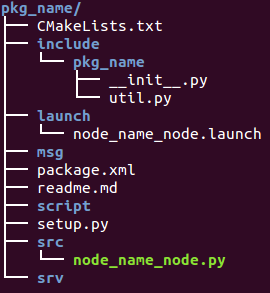
\includegraphics[width=\textwidth]{fig/pkg_tree.png}
		\end{column}
	\end{columns}
\end{frame}


\begin{frame}{Publisher Node Code Example with Timer}
	\framesubtitle{\texttt{publisher\_node\_timer.py}}
	\inputminted{python}{snippet/publisher_node_timer.py}
	\begin{itemize}
	\item Create a publisher: \pyinline{rospy.Publisher(topic_name,msg_type,queue_size)}
	\item Start a timer: \pyinline{rospy.Timer(duration,callback)}
	\end{itemize}
\end{frame}

\begin{frame}{Subscriber Node Code Example}
	\framesubtitle{\texttt{subscriber\_node.py}}
	\inputminted{python}{snippet/subscriber_node.py}
	\begin{itemize}
		\item Create a subscriber: \pyinline{rospy.Subscriber(topic_name,callback)}
	\end{itemize}
\end{frame}

\begin{frame}{Parameter Code Example}
	\framesubtitle{\texttt{publisher\_node\_param.py}}
	\inputminted{python}{snippet/publisher_node_param.py}
	% \begin{itemize}
	% 	\item Read parameter from parameter server:\\\pyinline{rospy.get_param(param_name,default_value)}
	% \end{itemize}
\end{frame}

\begin{frame}{Message Definition Examples}
	\begin{itemize}
		\item \texttt{Duckie.msg} defines the name, state, and pose of a duckie.
		\inputminted{python}{snippet/Duckie.msg}
		\item \texttt{DuckieList.msg} contains a list of duckies.
		\inputminted{python}{snippet/DuckieList.msg}
		\item Look up msg definition:\\\inline{rosmsg show pkg_name/msg_name}
	\end{itemize}
\end{frame}

\begin{frame}{Message Usage in Publisher Code Example}
	\framesubtitle{publisher\_node\_msg.py}
	\inputminted{python}{snippet/publisher_node_msg.py}
%	\todo[inline]{Use student name}
\end{frame}

\begin{frame}{Message Usage in Subscriber Code Example}
	\framesubtitle{subscriber\_node\_msg.py}
	\inputminted{python}{snippet/subscriber_node_msg.py}
\end{frame}


\begin{frame}{Resources}
	\begin{center}
	\inline{http://wiki.ros.org/}\\
	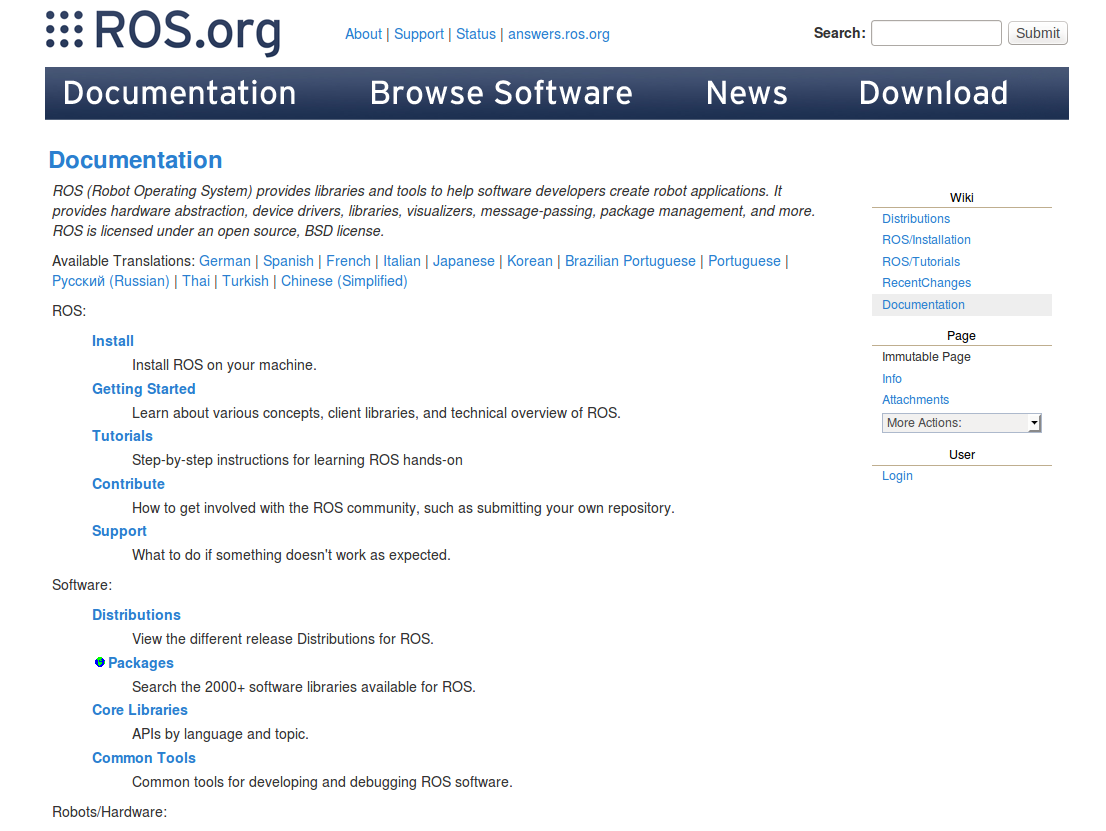
\includegraphics[width=\textwidth,keepaspectratio]{fig/ros_wiki.png}
	\end{center}
\end{frame}

\end{document}
